\section{Methodology}
\label{sec:methodology}

%\subsection{Background}
%\label{sec:background}

%\paragraph{Compartmental epidemiological models.}
%Compartmental models partition a host population into discrete states and model disease
%dynamics as a system of ordinary differential equations. The classical SIR model
%(Susceptible--Infected--Recovered) of Kermack and McKendrick has been extended to
%dozens of variants: SEIR (adding an Exposed/latent class), SEIRV (vaccination), multi-group
%(age-stratified, spatially coupled), vector-borne (host--vector compartments), and
%disease-specific structures~\cite{keeling2008modeling}. Despite their conceptual simplicity,
%published compartmental models vary substantially in which transitions, stratifications, and
%parameter conventions are made explicit, creating friction for model comparison and reuse.

%\paragraph{Implicit specification and reproducibility.}
%Reproducibility of a published compartmental model requires that a reader can recover
%the same states, flows, and parameter values the authors used. In practice, papers
%often leave conventional transitions unstated, embed parameters only in equations or
%supplements, or use ambiguous symbols whose meaning (e.g., population-level
%vs.\ individual-level contact rates) must be inferred from context~\cite{keeling2008modeling}.
%Calibration outputs, code, or posterior summaries may be separated from the ODE
%description in the main text. These patterns motivate treating alignment between paper
%promises, extracted structure, and an independent reference implementation as a measurable
%\emph{specification--validation gap}, which the remainder of this section operationalizes.

%\subsection{Pipeline overview}

Our framework consists of three phases: (\textit{i}) reference model analysis and
gold-standard construction, (\textit{ii}) LLM-assisted extraction of a draft model
from each paper PDF, and (\textit{iii}) gap detection, retrieval-augmented completion,
structural repair, and completeness scoring. All phases share a common XML
representation described below. Figure~\ref{fig:pipeline} illustrates the end-to-end
pipeline, where each phase produces structured artifacts consumed by the next.

\begin{figure*}[t]
  \centering
  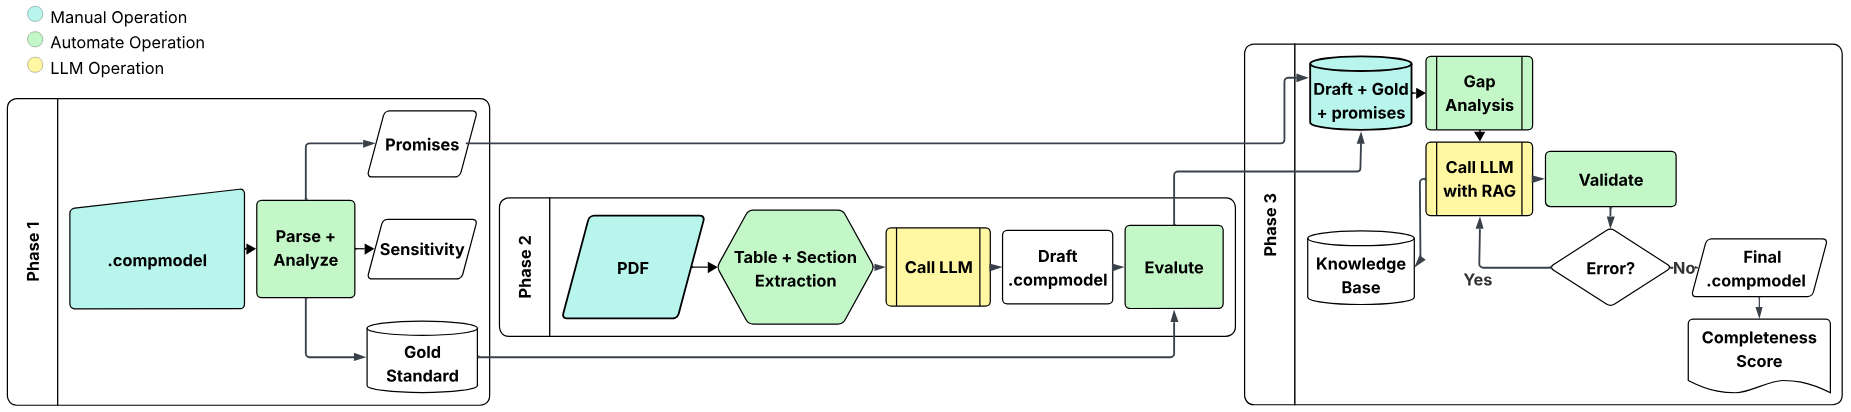
\includegraphics[width=\linewidth]{./figures/flow.png}
  \caption{Three-phase model completeness pipeline. Phase~1 builds reference models
  and structural baselines from existing \texttt{.compmodel} files. Phase~2 extracts
  a draft compartmental model from each paper PDF via LLM-assisted entity extraction.
  Phase~3 detects gaps against the gold-standard reference, fills them via RAG and
  LLM inference, and validates the result.}
  \label{fig:pipeline}
\end{figure*}

%\subsection{Artifact Representation: the \texttt{.compmodel} Format}
%\label{sec:compmodel}

All phases share a common XML representation for compartmental models, encoded in
\texttt{.compmodel} files under a well-defined metamodel. A model file contains:

\begin{itemize}[leftmargin=*]
  \item \textbf{Compartments} (\texttt{\textless{}compartments\textgreater{}}): each carries a
        \texttt{PrimaryName}, optional \texttt{SecondaryName} (stratification label),
        and an initial \texttt{population}. Stratified models (e.g., age-structured
        measles~\cite{Pokharel2024Measles}) encode strata as separate compartment
        entries with the stratum label in \texttt{SecondaryName}.
  \item \textbf{Outgoing flows} (nested under each compartment): typed as
        \texttt{ContactFlow} (mass-action infection, referencing a
        \texttt{contactCompartment} and a \texttt{contactRateParameter}) or
        \texttt{RateFlow} (first-order transition with a \texttt{rateParameter}).
        Flow endpoints reference other compartments by index
        (e.g., \texttt{target="//@compartments.2"}).
  \item \textbf{Parameters} (\texttt{\textless{}parameters\textgreater{}}): each has a \texttt{name},
        \texttt{type} (e.g., \textsc{Constant}), \texttt{expression} (numeric value
        or formula), \texttt{unit}, and \texttt{description}.
  \item \textbf{Groups} (\texttt{\textless{}groups\textgreater{}}): optional stratification dimensions
        (e.g., sex, age band) used to generate multi-group products.
\end{itemize}

Listing~\ref{lst:compmodel} shows a fragment for a two-compartment SIR contact flow.
The metamodel constrains which attributes are required per flow type, enabling
automated structural validation in Phase~3.

\begin{lstlisting}[caption={Fragment of a \texttt{.compmodel} file showing a ContactFlow
from Susceptible to Infectious parameterized by transmission rate $\beta$.},
label={lst:compmodel}, language=XML]
<compartments PrimaryName="Susceptible" population="9999">
  <outgoingFlows xsi:type="cm:ContactFlow"
    target="//@compartments.1"
    contactCompartment="//@compartments.1"
    contactRateParameter="//@parameters.0"/>
</compartments>
<parameters name="beta" type="CONSTANT"
  expression="0.3" unit="1/day"
  description="Transmission rate"/>
\end{lstlisting}

\subsection{Phase 1: Reference Model Analysis and Gold-Standard Construction}
\label{sec:phase1}

Phase~1 serves two roles: it \emph{parses} \texttt{.compmodel} files that were manually extracted to build structured JSON reports used as ground truth downstream, and it \emph{analyses} each model's structural and sensitivity properties.
To reduce subjectivity, gold models were derived from the equations and cross-checked
against reported simulations where available.

\textit{Structural Analysis.} The \texttt{CompModelParser} reads each XML file and
emits: compartment list with stratification info, parameter table with type and value,
and flow adjacency (source, target, type, associated parameter). These lists form
the \emph{gold standard} that Phases~2 and~3 compare against.

\textit{Paper Promise Extraction.} When a PDF is paired with a reference model,
Phase~1 runs pattern-based and LLM-assisted extraction to identify which model elements
(compartments, parameters, flows) the paper explicitly \emph{promises}, i.e., mentions
as part of its specification. The set of promises is stored in \texttt{paper\_promises.json}
and is used in Phase~3 to distinguish \emph{specification gaps} (promised but missing)
from \emph{reference gaps} (in gold but never mentioned).

\textit{Sensitivity Analysis.} For each model, Phase~1 runs a Morris elementary
effects screening~\cite{morris1991factorial} over the parameter space, producing per-parameter sensitivity
indices ($\mu^*$, $\sigma$) that identify which parameters most influence model
output. This metadata helps Phase~3 prioritize gap-filling by parameter importance.

\subsection{Phase 2: LLM-Assisted Extraction}
\label{sec:phase2}

Phase~2 turns an epidemiological PDF into a draft \texttt{.compmodel} without any manual
editing. We compare three commercial LLM backends: OpenAI GPT-5.4-mini~\cite{achiam2023gpt4},
Google Gemini~2.5~\cite{team2024gemini}, and Anthropic Claude Opus~4~\cite{anthropic2024claude}.
The pipeline has five steps.

\textit{Step 1 --- Text and Section Extraction.}
We employ GROBID~\cite{romary2015grobid} for high-fidelity header and section parsing, segmenting the PDF into distinct functional blocks (Abstract, Methods, Results). This ensures the LLM receives contextually isolated inputs rather than a monolithic text stream. To preserve mathematical notation and tabular data, we use Camelot~\cite{camelot2019} for table extraction and a Unicode-based normalization pass. This maintains symbol consistency (e.g., ensuring $\beta$ remains a consistent character across tables and prose) and prevents the structural corruption typical of standard PDF-to-text conversion.

\textit{Step 2 --- Paper Promise Detection.}
A prompt instructs the LLM to enumerate every compartment, parameter, and flow that the
paper \emph{claims} to include, using only the paper text. This produces
\texttt{paper\_promises.json}: a list of entity names plus supporting quotes.

\textit{Step 3 --- Entity Extraction.}
The LLM is asked to extract structured entities from the methods section, guided by the
epidemiological metamodel from Phase~1. For each compartment it extracts a primary name,
optional secondary name (stratum), and initial population; for each parameter, a name,
value, unit, and description; for each flow, a source compartment, target compartment,
type (contact or rate), and governing parameter. Flow endpoint names are snapped to
extracted compartment names using fuzzy matching (\texttt{SequenceMatcher} ratio
$\geq 0.78$) to avoid reference mismatches from minor label variation.

\textit{Step 4 --- Model Synthesis.}
Extracted entities are assembled into a \texttt{.compmodel} XML file. Flows referencing
compartments by name are resolved to index-based references. The resulting file is
\texttt{model\_draft.compmodel}.

\textit{Pipeline versions: original and enhanced.}
\label{sec:phase2versions}
We developed the Phase~2 extraction pipeline in two iterations to address systematic parsing failures. The \emph{original} pipeline used \texttt{PyPDF2}\footnote{\url{https://pypdf2.readthedocs.io/en/3.x/}} and \texttt{pdfplumber}\footnote{\url{https://github.com/jsvine/pdfplumber}} for basic text extraction, requiring manual two-column splitting and issuing independent LLM calls for compartments, flows, and parameters. This often resulted in fragmented models and lost context between text and tables. 

The \emph{enhanced} pipeline, adopted for all results reported in this paper, addresses three failure modes identified in early runs: 
(\textit{i})~\textbf{Structural Extraction} --- replaced \texttt{PyPDF2} with \textsc{grobid} and \texttt{Camelot} for section-aware parsing and table extraction (Step~1), preserving reading order and symbol integrity better than coordinate-based parsers; 
(\textit{ii})~\textbf{Unified Extraction} --- compartments, flows, and parameters are co-extracted in a single LLM call, improving cross-entity coherence and ensuring a flow's governing parameter is correctly linked; 
(\textit{iii})~\textbf{High-Density Context} --- \textsc{grobid}'s structured output automatically resolves hyphenation artifacts and removes non-content noise (page numbers, headers) before the LLM context window is assembled. 

%Across all providers, the enhanced pipeline raises mean compartment recall by $+10\%$ (Gemini) and $+4\%$ (Claude), and mean flow recall by $+12\%$ (Gemini) and $+5\%$ (Claude) over the original. A direct numerical comparison is presented in Section~\ref{sec:phase2results}.

\textit{Step 5 --- Evaluation.}
\label{sec:phase2eval}
The draft is compared to the Phase~1 gold standard using fuzzy string matching.
Names are normalized (lowercase, strip punctuation, map Greek letters to Latin:
$\beta \to \mathtt{beta}$, $\gamma \to \mathtt{gamma}$, etc.) and compared using
substring containment, with \texttt{SequenceMatcher}~\cite{python_difflib} ratio
$\geq 0.6$ as a fallback. Compartment and flow matching additionally checks
\emph{synonym groups} that encode epidemiological
conventions (\{Exposed, Latent, Incubating\}, \{Infectious, Infected, Symptomatic\},
\{Recovered, Removed, Immune\}). This makes match decisions
transparent, auditable, and fully reproducible with fixed thresholds and no
neural-model dependency.

The Phase~2 composite score used to select the best extraction per disease is
$\frac{1}{2}(\text{cF1} + \text{fF1}) \times 100$, where $cF1$ and $fF1$ are
compartment and flow F1 scores respectively.

\subsection{Phase 3: Gap Detection, Retrieval-Augmented Completion, and Structural Repair}
\label{sec:phase3}

Phase~3 takes the best Phase~2 draft (selected by composite score across three LLM backends)
and systematically closes its gaps. Gaps are first identified across three structural layers, then filled
by retrieval from the paper text (preferred, as fills are traceable), by optional LLM
inference (for residual gaps), or flagged for manual review.
The filled model is then validated against seven structural invariants and repaired where
possible. Finally, a five-component completeness score summarizes the result.
The sub-steps are as follows.

\textit{Three-Layer Gap Analysis.} We decompose the gap structure into three orthogonal layers:

\begin{enumerate}[leftmargin=*, label=\arabic*.]
  \item \textbf{Spec $\to$ Model} (\emph{promise gaps}): entities in
        \texttt{paper\_promises.json} but absent from \texttt{model\_draft.compmodel}.
        These are things the paper explicitly claims but the LLM failed to extract.
  \item \textbf{Model $\to$ Gold} (\emph{reference gaps}): entities in the gold-standard
        reference model but absent from the draft. These may be implicitly assumed by
        the paper and never directly stated.
  \item \textbf{Extras in model}: entities in the draft that have no counterpart in the
        gold. These are potential hallucinations or valid extensions not in the reference.
\end{enumerate}

All matching uses the same fuzzy protocol described in Section~\ref{sec:phase2eval}.
The three-layer breakdown is stored in \texttt{phase3\_threelayer\_gaps.json}.

\textit{Iterative Retrieval-Augmented Completion.}
Gap filling proceeds in two iterations to handle dependencies (e.g., a new compartment
added in iteration~1 enables a flow fill in iteration~2). Each iteration runs the
following priority tiers for each missing entity:

\noindent\textbf{Tier~1 -- RAG fill}: A lexical RAG index over the paper's text chunks
(chunk size 2000 chars, 300-char overlap) is queried by entity name and synonyms.
If a matching passage with a numeric value is found, the value is used directly. The
same database is queried for structural clues (e.g., a textual description of a
transition rate).

\noindent\textbf{Tier~2 -- Spec-entity fill} (first iteration only): Entities extracted
but not yet placed in the model (from \texttt{extracted\_entities.json}) are used to
fill matching gaps by name similarity.

\noindent\textbf{Tier~3 -- LLM inference} (optional, \texttt{--inference} flag): For
gaps that remain unfilled after RAG, the LLM is prompted with the paper text and the
gap description to infer a plausible value or structure. This tier is disabled in
\emph{rag\_only} mode to assess pure retrieval performance.

\noindent\textbf{Tier~4 -- Flag}: Remaining unfilled gaps are flagged for manual review
with severity annotation (critical / high / medium / low).

Fills are applied to produce \texttt{model\_filled.compmodel}. Each fill record carries
a \texttt{source} tag (\texttt{rag}, \texttt{spec\char`\_entity}, \texttt{inference}, or
\texttt{flagged}) used in traceability scoring.

\textit{Structural Validation.}
The filled model is checked against seven structural invariants, independent of any
gold standard:

\begin{enumerate}[leftmargin=*, label=\arabic*.]
  \item \textbf{Self-referential flow}: a ContactFlow whose source, target, and
        contact compartment are all the same compartment, implying an impossible mass-action term.
  \item \textbf{Orphaned parameters}: a parameter declared in
        \texttt{\textless{}parameters\textgreater{}} but
        not referenced by any flow's \texttt{rateParameter} attribute, meaning it has
        no effect on dynamics.
  \item \textbf{Uniform parameter collapse}: a single parameter assigned to
        \emph{all} flows, indicating the LLM reused one entry rather than assigning
        distinct rates.
  \item \textbf{Zero population everywhere}: all compartments carry population~0,
        making simulation degenerate.
  \item \textbf{Broken flow chain}: a non-terminal compartment (not dead/recovered)
        has no outgoing flow, creating a sink that traps individuals indefinitely.
  \item \textbf{Missing birth source}: susceptible compartments lack any population
        initialization, preventing simulation from starting.
  \item \textbf{Parameter layer contamination}: parameter expressions contain
        Bayesian or posterior inference keywords (e.g., ``posterior mean'', ``MCMC''),
        indicating the LLM confused estimation outputs with model inputs.
\end{enumerate}

Errors are classified by severity (critical, high, medium, low) to prioritize repairs.
The pre-repair error profile is stored in \texttt{phase3\_structural\_before.json}.

\textit{Structural Repair.}
Each error class corresponds to a \emph{deterministic} failure mode, where the
correct fix is unambiguous given the model's XML schema and the error type (e.g., a
zero-population compartment always needs a nominal value or a contaminated parameter
expression always needs its Bayesian term cleared). Rule-based repair is therefore
appropriate here. The rules are not heuristic workarounds but direct structural
corrections implied by the schema invariants.
The empirical justification is in Table~\ref{tab:structural}. Deterministic error classes
(uniform parameter collapse, zero population) resolve at 100\%, while structurally
ambiguous classes (orphaned parameters, self-referential flows) resolve at lower rates,
confirming that the rules are neither over- nor under-specified.
The repairs applied for each error class are:

\begin{itemize}[leftmargin=*]
  \item \textit{Zero population / missing birth source}: set the susceptible
        compartment's population to a nominal value (1000) to enable simulation.
  \item \textit{Self-referential flow}: if an Exposed/Latent intermediate compartment
        exists, redirect the flow target through it; otherwise, annotate the flow
        description to flag the issue.
  \item \textit{Uniform parameter collapse}: reassign each flow's rate parameter by
        semantic category matching (transmission, recovery, mortality, progression)
        using the parameter description and flow endpoint names.
  \item \textit{Orphaned parameter}: in a first pass, assign the parameter to any flow
        that currently has no rate parameter and whose semantic category matches; in a
        second pass (only when no parameter collapse is being resolved simultaneously),
        swap a clearly mismatched existing assignment if the orphaned parameter is a
        much better category match (description similarity $> 0.6$).
  \item \textit{Broken flow chain}: add a \texttt{RateFlow} from the stranded
        compartment to the most semantically appropriate next compartment
        (Infectious~$\to$~Recovered, etc.).
  \item \textit{Parameter contamination}: clear Bayesian inference expressions from
        the parameter value field.
\end{itemize}

Repairs run for up to two iterations, re-validating after each pass to catch
dependencies. The repaired model is written to \texttt{model\_repaired.compmodel} and
the repair log to \texttt{phase3\_repair\_log.json}.

\textit{Completeness Score.}
\label{sec:completeness}
We define a composite \emph{completeness score} $\mathcal{C} \in [0, 100]$ as a
weighted sum of five components:

\begin{equation}
  \mathcal{C} = 25 \cdot G + 25 \cdot R + 20 \cdot T + 15 \cdot A + 15 \cdot S
  \label{eq:completeness}
\end{equation}

\noindent where each term is a fractional score in $[0,1]$.
The weights are designed to reflect a coverage-first notion of model completeness:
gap reduction ($G$) and reference agreement ($R$) receive the highest weight as
they measure recovery of the intended model structure, which is the primary objective
of completeness auditing. Traceability ($T$) captures whether recovered elements are
supported by evidence in the paper text, distinguishing verifiable specification from
inferred reconstruction. Parameter accuracy ($A$) and structural integrity ($S$)
capture numerical correctness and internal consistency, which are secondary to
coverage but necessary to ensure that a recovered model is well-formed.
The weights are set a priori to reflect this hierarchy, and we confirm in
Section~\ref{sec:threats} that results are robust under alternative weight
configurations.

\begin{itemize}[leftmargin=*]
  \item $G$ — \textbf{Gap reduction} (25\%): fraction of gaps closed after Phase~3,
        $(\text{gaps}_\text{before} - \text{gaps}_\text{after}) / \text{gaps}_\text{before}$.
  \item $R$ — \textbf{Reference agreement} (25\%): mean entity recall of the
        repaired model against the gold standard.
  \item $T$ — \textbf{Fill traceability} (20\%): fraction of fills whose source
        is a retrieved paper passage (\texttt{rag} or \texttt{spec\_entity});
        LLM-inferred or flagged fills score 0, directly penalizing unverifiable content.
  \item $A$ — \textbf{Parameter accuracy} (15\%): fraction of parameters whose
        numeric value is within 10\% of the gold value.
  \item $S$ — \textbf{Structural integrity} (15\%): error reduction rate,
        $1 - e_\text{after}/e_\text{before}$, measuring how well rule-based repair
        resolves detected inconsistencies.
\end{itemize}

Together, $G$ and $R$ measure \emph{coverage} (did we find the right things?), $T$
measures \emph{auditability} (can we point to the paper text?), $A$ measures
\emph{accuracy} (are the numbers right?), and $S$ measures \emph{consistency}
(is the model internally valid?). A score of 100 would require a paper that is
fully explicit, fully specified, and structurally consistent---a standard no paper
in our dataset meets.

\textit{Mode Comparison and Best-Model Selection.}
Phase~3 runs in three modes per disease: \emph{rag\_only} (Tiers~1--2 only),
\emph{llm\_only} (Tier~3 only, no RAG), and \emph{both} (all tiers). The winner mode
is selected by: fewest gaps $\to$ highest parameter accuracy $\to$ highest mean
compartment/flow F1. This ablation isolates the contribution of retrieval versus
LLM inference.
